\startslide
\commonframe
\mbox{}

\begin{tikzpicture}[remember picture,overlay]
  \slidetitle{Вариант на PostgreSQL}

  \node[anchor=north west] at ([xshift=8.55cm,yshift=-1.72cm]current page.north west) {%
    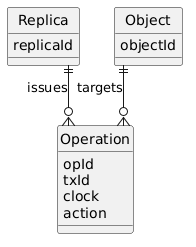
\includegraphics[width=5.15cm]{../postgresql/resources/diagram.png}%
  };

  \node[
    anchor=north west,
    fill=softbg,
    rounded corners=10pt,
    text width=6.2cm,
    inner xsep=0.35cm,
    inner ysep=0.28cm,
    align=left
  ] at ([xshift=0.95cm,yshift=-1.78cm]current page.north west) {%
    {\fontsize{8.8}{10.0}\selectfont
    \textbf{Модель хранения}\\[0.10cm]
    Три таблицы: \texttt{replicas}, \texttt{objects}, \texttt{operations}.\\
    Журнал операций хранится как \textbf{append-only} набор независимых строк.}%
  };

  \node[
    anchor=north west,
    fill=softgray,
    rounded corners=10pt,
    text width=6.2cm,
    inner xsep=0.30cm,
    inner ysep=0.24cm,
    align=left
  ] at ([xshift=0.95cm,yshift=-4.22cm]current page.north west) {%
    {\fontsize{8.8}{9.8}\selectfont
    \textbf{Сильные стороны}\\
    • строгая схема и ссылочная целостность;\\
    • удобные выборки по \texttt{opId}, \texttt{txId}, \texttt{objectId}.\\[0.16cm]
    \textbf{Ограничения}\\
    • часть структуры остаётся внутри \texttt{JSONB};\\}%
  };

\end{tikzpicture}

\footerband{4}
